\section{Τοπολογική Ανάλυση Χώρου}
\label{section:map_annotation}

Στο πρώτο μέρος της εργασίας αυτής αναλύεται ο διδιάστατος χάρτης του χώρου με στόχο τον εντοπισμό των διάφορων δωματίων που αποτελούν τον χώρο αυτό. Για την επίτευξη αυτού χρησιμοποιούνται ορισμένοι αλγόριθμοι που παρουσιάζονται στην συνέχεια. 

\subsubsection{Αλγόριθμος Brushfire}
\label{subsection:brushfire_algorithms}

Αρχικά, υλοποιήθηκε η πιο απλή αλλά και σημαντική εκδοχή του αλγορίθμου brushfire \ref{section:brushfire_theory}, η οποία είναι η εύρεση του πεδίου brushfire των εμποδίων του OGM. Χρησιμοποιείται ως αρχικό υποσύνολο σημείων το σύνολο των εμποδίων του OGM και υπολογίζεται για κάθε σημείο του ελεύθερου χώρου η απόσταση του από το κοντινότερο του εμπόδιο. Η διαδικασία, λοιπόν, εκκινεί από τα εμπόδια και εξαπλώνεται συνεχώς σε όλα τα γειτονικά σημεία που δεν έχει διαδοθεί. Η επαναληπτική αυτή μέθοδος μπορεί να γίνει πιο κατανοητή από το \autoref{fig:brushfire_example}. Όπως φαίνεται, το κύμα ξεκινάει περιμετρικά των εμποδίων και εξαπλώνεται κατά ένα σημείο την φορά. Η διαδικασία συνεχίζεται μέχρι να μην μπορεί να πραγματοποιηθεί άλλη εξάπλωση στον χώρο, που σημαίνει ότι και κάλυψε ολόκληρο τον χώρο.


\begin{figure}[!htb]
    \centering
    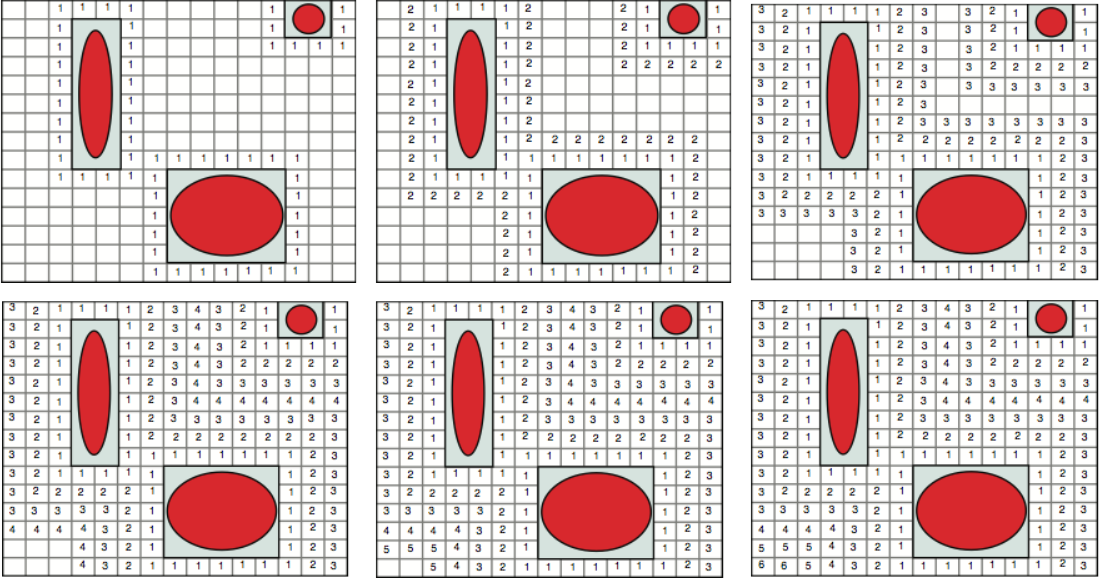
\includegraphics[width=\textwidth]{./images/chapter5/brushfire0.png}
    \caption{Παράδειγμα Brushfire}
    Πηγή: \href{http://roboscience.org/book/html/Planning/Brushfire.html}{http://roboscience.org/book/html/Planning/Brushfire.html}
    \label{fig:brushfire_example}
\end{figure}



\begin{algorithm}[!htb]
\caption{Obstacle Brushfire}
\label{alg:obstacle_brushfire}
\begin{algorithmic}[1]
    \Function{obstacleBrushfire}{ogm}
        \State $brushfire = np.zeros(ogm.shape)$
        \State $brushfire[ogm > 49] = 1$
        \State $brushfire[ogm == -1] = -1$
        \State $step = 1$
        \State $changed = 1$
        \While{$changed == 1$}
            \State $changed = 0$
            \For{$i$ = 1 to ($brushfire.width$ - 1)}
                \For{$j$ = 1 to ($brushfire.height$ - 1)}
                    \If{$brushfire[i][j] == 0$ and a neighbor's brushfire value is equal to step}
                        \State $brushfire[i][j] = step + 1$
                        \State $changed = 1$
                    \EndIf
                \EndFor
            \EndFor
            \State $step += 1$
        \EndWhile
        \State \Return $brushfire$
            
\end{algorithmic}
\end{algorithm}

Ο brushfire εμποδίων παρουσιάζεται στο \ref{alg:obstacle_brushfire}. Στις γραμμές 2-4 το πεδίο brushfire ορίζεται έτσι ώστε να έχει τις ίδιες διαστάσεις με το ogm, αρχικά με μηδενικές τιμές στον ελεύθερο χώρο, 1 στα εμπόδια και -1 στα άγνωστα σημεία. Για όσο συμβαίνει η εξάπλωση εξετάζονται όλα τα σημεία του brushfire. Εαν σε κάποιο ελεύθερο σημείο δεν έχει φτάσει ακόμα το κύμα αλλά έχει φτάσει σε έναν γείτονα του στην προηγούμενη επανάληψη με τιμή $step$, τότε και στο τρέχον σημείο ανανεώνει το brushfire με τιμή $step + 1$. Η διαδικασία επαναλαμβάνεται εως ότου δεν επέλθει καμία ανανέωση στον πίνακα $brushfire$, δηλαδή μέχρι την πλήρη εξάπλωση των τιμών.

\subsubsection{Υπολογισμός GVD}
\label{subsection:gvd_algorithms}
Εξίσου χρήσιμο με το $brushfire$ του χάρτη είναι και το GVD του. Αυτό υπολογίζεται χρησιμοποιώντας τη μέθοδο skeletonize\footnote{\href{https://scikit-image.org/docs/dev/auto_examples/edges/plot_skeleton.html}{https://scikit-image.org/docs/dev/auto\_examples/edges/plot\_skeleton.html}} της βιβλιοθήκης της skimage της Python. Το GVD έχει τις ίδιες διαστάσεις με το αντίστοιχο OGM και οι τελικές του τιμές θα είναι 1 στα σημεία που ανήκουν σ' αυτό και 0 σε όλα τα υπόλοιπα. Στην μέθοδο skeletonize εισάγεται ως δυαδική εικόνα ο ελεύθερος χώρος του OGM. Όπως φαίνεται στην εντολή 3 του αλγορίθμου \ref{alg:gvd} χρησιμοποιούνται ως είσοδο τα σημεία που έχουν τιμή brushfire μεγαλύτερη από 5, δηλαδή όλα τα ελεύθερα σημεία εκτός από αυτά που είναι πάρα πολύ κοντά στα εμπόδια. Ο OGM πολλές φορές περιέχει ατέλειες πολύ κοντά στα εμπόδια λόγω αστοχίας της διαδικασίας του SLAM. Χαρακτηριστικό παράδειγμα είναι η περίπτωση να θεωρεί ως ελεύθερο χώρο σημεία πίσω από τον τοίχο, εκτός του χώρου, που κανονικά θα έπρεπε να θεωρούνται άγνωστα. Προκειμένου να μην επηρεάσουν τη διαδικασία υπολογισμού του GVD, λαμβάνονται υπόψη τα σημεία που έχουν μια στοιχειώδη απόσταση από τα εμπόδια.


\begin{algorithm}[!ht]
\caption{GVD}
\label{alg:gvd}
\begin{algorithmic}[1]
    \Function{gvd}{brushfire}
        \State $voronoi = np.zeros(brushfire.shape)$
        \State $voronoi[brushfire >= 5] = 1$
        \State $voronoi = skimage.morphology.skeletonize(voronoi)$
        \State \Return $voronoi$
\end{algorithmic}
\end{algorithm}



\subsection{Υπολογισμός τοπολογικού γράφου του χώρου}
\label{subsection:find_topology}

Το GVD ενός χάρτη περιέχει σημαντικές πληροφορίες για το περιβάλλον. Κρύβει μέσα του τόσο τα όρια των δωματίων όσο και την δομή τους. Επομένως, χρειάζεται να εξαχθούν σημεία που περιέχουν αυτές τις πληροφορίες. Πιο σημαντικοί είναι οι κόμβοι που αντιστοιχούν στις πόρτες του χώρου, καθώς με αυτούς μπορεί να διαχωριστεί αποτελεσματικά ο χάρτης στα δωμάτια του. Η μέθοδος βασίστηκε σε μια αντίστοιχη μελέτη γνωστού χώρου που είχε πραγματοποιηθεί στο \cite{sikoudi}. 

Η διαδικασία που υλοποιήθηκε αναλύεται στη συνέχεια. Καταρχάς, κάθε σημείο του GVD μπορεί να έχει από ένα έως τέσσερα γειτονικά σημεία τα οποία ανήκουν και αυτά στο GVD. Ανάλογα μάλιστα με το πλήθος των γειτόνων, μπορούν να εξαχθούν πληροφορίες για το κάθε σημείο. Έτσι, παρατηρώντας και το \autoref{fig:gvd_neighbors_example} τα σημεία με έναν μόνο γείτονα βρίσκονται στις άκρες του GVD, δηλαδή σε περιοχές που πλησιάζουν σε εμπόδια, όπως οι γωνίες των δωματίων και επισημαίνονται με κίτρινους κύκλους. Αντίστοιχα, τα σημεία με τρεις ή τέσσερις γείτονες βρίσκονται σε πιο κεντρικά, όσον αφορά τις αποστάσεις από τα εμπόδια, σημεία ή σε σημεία διακλάδωσης, όπως η περιοχή μπροστά από μια πόρτα, όπου και το διάγραμα διακλαδίζεται και επισημαίνονται με κόκκινους κύκλους. Το σημείο που αντιστοιχεί σε πόρτα επισημαίνεται με πράσινο χρώμα και όπως φαίνεται έχει δύο γείτονες. Όλοι αυτοί οι κόμβοι πρέπει να εξαχθούν από το GVD για να δημιουργηθεί ο τοπολογικός γράφος του χώρου.

Πρώτα, σαρώνεται ο χώρος, ώστε να βρεθούν όλα τα σημεία του GVD με έναν, τρεις ή περισσότερους γείτονες. Αυτά αν και δεν χρειάζονται για την εύρεση των πορτών και τον διαχωρισμό των δωματίων, μπορούν να χρησιμοποιηθούν για άλλους λόγους, όπως παρουσιάζεται στο \ref{section:room_classification}.

Έπειτα, πρέπει να μελετηθούν τα σημεία με δύο γείτονες για να εξαχθούν οι κόμβοι οι οποίοι είναι πιθανό να αποτελούν πόρτες στον χώρο. Για την επίτευξη αυτού θα χρησιμοποιηθεί η τιμή brushfire που έχουν αυτά τα σημεία. Συγκεκριμένα, τα σημεία πόρτες παρουσιάζουν τοπικό ακρότατο στην τιμή brushfire τους. Αυτό γίνεται εύκολα αντιληπτό εαν σκεφτεί κανείς πως για να περάσει το ρομποτικό όχημα, αλλά και ένας άνθρωπος, από μια πόρτα θα πλησιάσει τα εμπόδια, θα φτάσει σε μια ελάχιστη απόσταση ακριβώς στην ευθεία της πόρτας και μετά θα αρχίσει να απομακρύνεται από αυτά. Η ιδιότητα αυτή είναι καθοριστική, καθώς οι υποψήφιες πόρτες μπορούν να βρεθούν, εαν υπολογιστούν τα τοπικά ελάχιστα του brushfire στα σημεία που ανήκουν στο GVD και έχουν δύο γείτονες. Αυτό φαίνεται και στο \autoref{fig:brushfire_minimum_example} όπου έχουν επισημανθεί τα σημεία που ανήκουν στο GVD, ενώ για κάθε σημείο έχει γραφεί το brushfire του. Πράγματι τα σημεία με πράσινο αποτελούν το τοπικό ελάχιστο του brushfire πάνω στο GVD. 

Η διαδικασία που υλοποιήθηκε ελέγχει για κάθε σημείο του GVD με δύο γείτονες εαν έχει την ελάχιστη brushfire τιμή σε μια περιοχή 20x20 γύρω απ' αυτό, συγκρίνοντας μόνο σημειά που ανήκουν στο διάγραμμα Voronoi. Έτσι, βρίσκονται τα τοπικά ελάχιστα τα οποία, όμως, χρειάζονται περαιτέρω επεξεργασία. Όπως φαίνειται και στο \ref{fig:brushfire_minimum_example} για κάθε πόρτα περισσότερα από ένα σημεία αποτελούν τοπικό ελάχιστο, καθώς ο αλγόριθμος brushfire εξαπλώνεται και στα οχτώ γειτονικά του σημεία. Για την αναγωγή κάθε τοπικού ελαχίστου στο πιο αντιπροσωπευτικό της πόρτας, ομαδοποιούνται τα σημεία ανά γειτονιές και κρατιέται το μεσαίο από κάθε ομάδα ως υποψήφιος κόμβος πόρτας.

\begin{figure}[!htb]
    \centering
    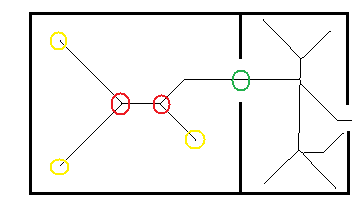
\includegraphics[width=0.5\textwidth]{./images/chapter5/rooms_3_gvd_1_3_neighbors_pinned.png}
    \caption{Κόμβοι τοπολογικού γράφου}
    \label{fig:gvd_neighbors_example}
\end{figure}


\begin{figure}[!htb]
    \centering
    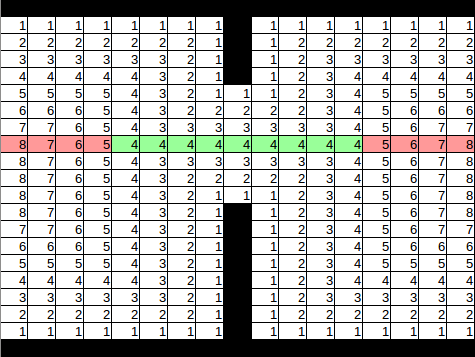
\includegraphics[width=0.5\textwidth]{./images/chapter5/brushfire_gvd_example.png}
    \caption{Τοπικό Ελάχιστο Brushfire στις πόρτες}
    \label{fig:brushfire_minimum_example}
\end{figure}


Η διαδικασία παρουσιάζεται στον αλγόριθμο \ref{alg:topological_nodes} και χρησιμοποιεί τα ήδη υπολογισμένα πεδία brushfire και GVD του χώρου. Στις εντολές 2-14 γίνεται η πρώτη εξαγωγή χρήσιμων κόμβων από το GVD. Στη συνέχεια στις εντολές 16-26 ομαδοποιούνται οι κόμβοι με δύο γείτονες που βρίσκονται στην ίδια γειτονιά, δηλαδή που αντιστοιχούν στην ίδια πόρτα, και κρατιέται ο μεσαίος κόμβος ως υποψήφιος κόμβος πόρτας.



\begin{algorithm}[!htb]
\caption{Topological Nodes}
\label{alg:topological_nodes}
\begin{algorithmic}[1]
    \Function{topologicalNodes}{brushfire, gvd}
        \State $nodes = []$
        \For{every point $(x,y)$ of gvd, where $gvd == 1$}
            \State count gvd neighbors of point $(x,y)$
            \If{number of neighbors is 1, 3 or 4}
                \State $nodes.append((x,y))$
            \EndIf
            \If{number of neighbors is 2}
                \State Check if $brushfire[x,y]$ is minimum in a 20x20 area
                \If{ $brushfire[x,y]$ is min }
                    \State $nodes.append((x,y))$
                \EndIf
            \EndIf
        \EndFor
        \State \Comment{Recheck nodes with 2 neighbors to keep one point of each neighborhood}
        \State $final\_nodes = []$
        \State add all nodes that don't have 2 neighbors to $final\_nodes$
        \State Group nodes with 2 neighbors to lists of points of same line
        \For{each list of points}
            \If{number of nodes in list is odd}
                \State add middle point to $final\_nodes$
            \Else
                \State add first of the two middle points to $final\_nodes$
            \EndIf
        \EndFor
        \State \Return $final\_nodes$
\end{algorithmic}
\end{algorithm}

Τα ενδιάμεσα αποτελέσματα παρουσιάζονται και στα επόμενα σχήματα. Συγκεκριμένα, οι μικρές ευθείες των τοπικών ελαχίστων παρουσιάζονται στο \ref{fig:rooms_3_door_lines}, όπου με μπλε σημειώνονται τα σημεία που πράγματι είναι κοντά σε μια πόρτα και με πράσινο σημεία που ενώ είναι ακρότατα του χάρτη, δεν αντιστοιχούν σε κάποια πόρτα. Μάλιστα, αυτά τα σημεία αποτελούν τοπικά μέγιστα του χώρου. Στην πράξη, λοιπόν, αν και ο αλγόριθμος αναζητάει τοπικά ελάχιστα μόνο, είναι πολύ πιθανό να βρει και τοπικά μέγιστα, καθώς για κάθε σημείο του GVD η brushfire τιμή του συγκρίνεται με τις γύρω 20x20 τιμές. Αυτό σημαίνει ότι σε περιπτώσεις που παρουσιάζονται και τοπικά μέγιστα, εαν αυτά αποτελούνται από περισσότερα από 20 σειριακά σημεία, θα κρατηθούν ορισμένα από αυτά. Για να καταλάβει ο αλγόριθμος ότι πρόκειται πράγματι για μέγιστο και όχι ελάχιστο θα χρειαζόταν να ελέγξει μια μεγαλύτερη περιοχή από τα 20x20 σημεία που καλύπτει ήδη, κάτι που όμως δεν θα έλυνε αποτελεσματικά το πρόβλημα για κάθε χώρο. Πάντα θα υπάρχει ένα περιβάλλον που θα χρειάζεται μεγαλύτερο πεδίο σύγκρισης των τιμών brushfire με το τρέχον σημείο. Το πρόβλημα διαχωρισμού των πραγματικών πορτών, λοιπόν, θα αντιμετωπιστεί στην επόμενη υποενότητα με μια διαφορετική διαδικασία.

Στο \autoref{fig:rooms_3_doors} παρουσιάζονται τα αντιπροσωπευτικά σημεία κάθε μικρού ευθύγραμμου τμήματος του προηγούμενου σχήματος με τα αντίστοιχα χρώματα. Οι κόμβοι αυτοί αποτελούν το σύνολο των υποψήφιων κόμβων πόρτας του χώρου. 

Τέλος, στο \autoref{fig:rooms_3_nodes_with_doors} παρουσιάζονται όλοι οι κόμβοι που επιστρέφει ο αλγόριθμος \ref{alg:topological_nodes}. Με μπλε εμφανίζονται οι τελικές πόρτες και με κόκκινο όλα τα υπόλοιπα σημεία στα εσωτερικά των δωματίων.


\begin{figure}{\textwidth} 
    \centering
    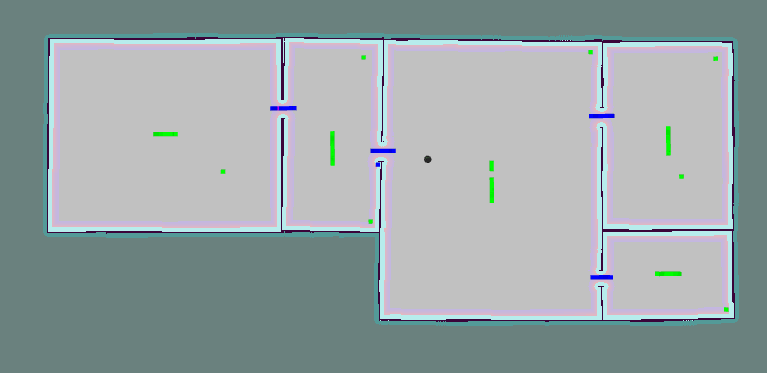
\includegraphics[width=0.7\textwidth]{./images/chapter5/rooms_3_door_lines.png}
    \caption{Ευθείες με Κόμβους Τοπικών Ακροτάτων}
    \label{fig:rooms_3_door_lines}
\end{figure}
\begin{figure}{\textwidth} 
    \centering
    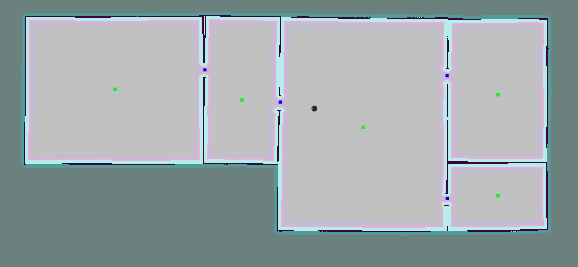
\includegraphics[width=0.7\textwidth]{./images/chapter5/rooms_3_doors.png}
    \caption{Υποψήφιοι Κόμβοι Πόρτες}
    \label{fig:rooms_3_doors}
\end{figure}
\begin{figure}{\textwidth} 
    \centering
    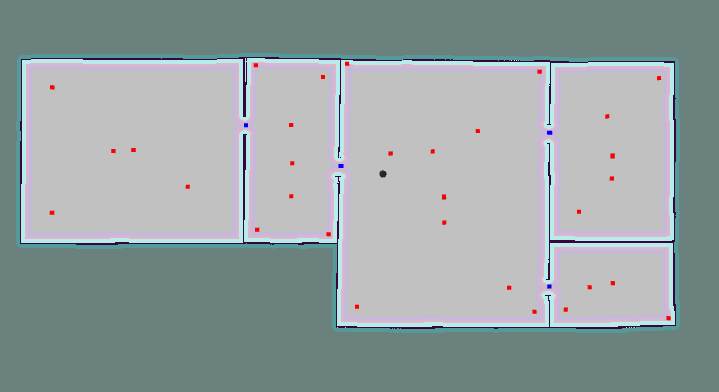
\includegraphics[width=0.7\textwidth]{./images/chapter5/rooms_3_nodes_with_doors.png}
    \caption{Τελικοί Κόμβοι Τοπολογικού Γράφου του Χώρου}
    \label{fig:rooms_3_nodes_with_doors}
\end{figure}


\subsection{Ορισμός των Κόμβων Πόρτας}
\label{subsection:find_door_nodes}

Το επόμενο βήμα της διαδικασίας είναι η εύρεση των πραγματικών πορτών του χώρου. Ως πιθανοί κόμβοι πόρτας λαμβάνονται όλοι οι κόμβοι της προηγούμενης διαδικασίας που έχουν δύο ακριβώς γείτονες στο GVD. Όπως αναλύθηκε νωρίτερα, υπάρχουν περισσότεροι υποψήφιοι κόμβοι από τις πραγματικές πόρτες ακόμη και σε περιβάλλοντα με απλή εσωτερική δομή. Φυσικά, όσο περισσότερα εμπόδια περιέχει ο χώρος, τόσα περισσότερα πιθανά σημεία πόρτας υπάρχουν. 

Η εύρεση των πραγματικών πορτών από το σύνολο των υποψήφιων βασίζεται σε μια σημαντική ιδιότητα κάθε πόρτας. Οι κόμβοι των πραγματικών πορτών βρίσκονται ενδιάμεσα δύο εμποδίων, των δύο τοιχών της πόρτας. Τα δύο αυτά σημεία σχηματίζουν, μάλιστα, μια ευθεία στον χώρο στην προέκταση της οποίας υπάρχει σημαντικό ποσοστό κατειλλημένου χώρου από την προέκταση των εμποδίων. Στόχος είναι να βρεθεί ένα κατάλληλο κατώφλι προσαρμοσμένο στον κάθε χάρτη, ώστε να συγκριθούν τα ποσοστά όλων των κόμβων με αυτό και να επιλεγούν μόνο αυτοί που έχουν μεγαλύτερο ποσοστό από το όριο αυτό.

Στο \autoref{fig:door_line_example} παρουσιάζονται τρεις διαφορετικές περιπτώσεις κόμβων που είναι υποψήφιοι να είναι κόμβοι πόρτες. Οι κόμβοι αυτοί έχουν κόκκινο χρώμα, ενώ τα σημεία που αποτελούν τα πιο κοντινά εμπόδια έχουν μπλε χρώμα. Η ευθεία των εμποδίων εμφανίζεται με διακεκομμένη πράσινη γραμμή. Στο πρώτο σχήμα, ο υποψήφιος κόμβος πόρτας βρίσκεται κοντά σε μια γωνία του δωματίου. Δεν αποτελεί σημείο πόρτας διότι δεν βρίσκεται ανάμεσα στα δύο σημεία των εμποδίων, δηλαδή δεν βρίσκεται πάνω στην πράσινη ευθεία. Στο δεύτερο σχήμα, ο υποψήφιος κόμβος αποτελεί σημείο της ευθείας αυτής. Όμως, τα σημεία που ανήκουν στην ευθεία κατά κύριο λόγο αποτελούν ελεύθερα σημεία του χώρου, πράγμα που σημαίνει ότι δεν υπάρχουν οι αναμενόμενοι τοίχοι στην προέκταση των εμποδίων. Τέλος, στο τρίτο σχήμα παρουσιάζεται η περίπτωση της πραγματικής πόρτας. Είναι εύκολα διακριτό το γεγονός ότι μεγάλο ποσοστό των σημείων που ανήκουν στην εν λόγω ευθεία είναι σημεία εμποδίων.


\begin{figure}[!htb]
    \centering
    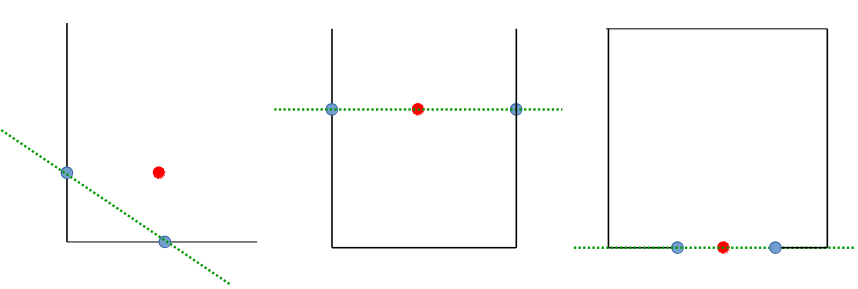
\includegraphics[width=0.9\textwidth]{./images/chapter5/door_line_example.png}
    \caption{Παραδείγματα Ελέγχου Κόμβων Πόρτας}
    \label{fig:door_line_example}
\end{figure}



\medskip
Ο αλγόριθμος παρουσιάζεται σε αναλυτική μορφή στο \ref{alg:find_door_nodes}. Η διαδικασία συνοψίζεται για κάθε υποψήφιο κόμβο στα παρακάτω βήματα:
\begin{itemize}
    \setlength\itemsep{-0.2em}
    \item Εύρεση κοντινότερων εμποδίων του κόμβου
    \item Έλεγχος πλήθους αυτών των σημείων
    \item Εύρεση της ευθείας των σημείων αυτών και έλεγχος της εγγύτητας του κόμβου με αυτήν
    \item Μέτρηση ποσοστού κάλυψης στο OGM σε ένα πεπερασμένο μήκος της ευθείας αυτής
    \item Υπολογισμός κατωφλιού απόφασης
    \item Σύγκριση ποσοστού με κατώφλι αποδοχής κόμβου ως πόρτα
\end{itemize}


Το πρώτο βήμα κάνει χρήση της συνάρτησης \ref{alg:closestObstacleBrushfire} η οποία δέχεται ως είσοδο ένα OGM και τον τρέχοντα κόμβο και εκτελεί brushfire με αρχή το σημείο αυτό, μέχρι να φτάσει η εξάπλωση στο πρώτο εμπόδιο. Τότε, η διαδικασία εκτελείται για άλλη μια επανάληψη και στη συνέχεια τερματίζεται. Η ύπαρξη της μιας παραπάνω φοράς είναι αναγκαία, καθώς σε περίπτωση που σε μια πόρτα μεσολαβεί άρτιος αριθμός ελεύθερων σημείων, ο κόμβος της πόρτας θα βρίσκεται στην μια πλευρά πιο κοντά κατά ένα pixel. Με τον τρόπο αυτό, όμως, θα εντοπιστούν και οι δύο πλευρές των εμποδίων. Στη συνέχεια, τα εμπόδια όπου έφτασε ο brushfire ομαδοποιούνται σε γειτονικά και επιλέγεται να επιστραφεί από κάθε ομάδα το σημείο που είναι πιο κοντά στον κόμβο εκκίνησης. Η εντολή αυτή καλείται στην γραμμή 4. 

Έπειτα, πραγματοποιείται ο έλεγχος του πλήθους των σημείων των εμποδίων στην γραμμή 5. Το επόμενο βήμα υλοποιείται με τις εντολές 7-11. Μετά μετράται το ποσοστό κάλυψης των σημείων της ευθείας. Πολλές φορές όμως ένα OGM μπορεί να περιέχει ατέλειες. Γι αυτό τον λόγο ο αλγόριθμος χρησιμοποιεί σημεία που είναι γύρω από την ευθεία. Συγκεκριμένα, χρησιμοποιείται το ευθύγραμμο τμήμα των δύο σημείων των εμποδίων της εντολής 4 με 50 pixels επέκταση προς κάθε πλευρά. Επίσης, το πλάτος της ευθείας από 1 pixel αυξάνεται στα 5 pixel. Με τον τρόπο αυτό εξασφαλίζεται ότι οι γύρω τοίχοι θα βρίσκονται μέσα στην περιοχή που προσμετράται στο ποσοστό κάλυψης. Άλλωστε το πάχος των τοιχών στα συνήθη OGM είναι μεγαλύτερο του ενός pixel, συνεπώς οι επεκτάσεις θα οδηγήσουν σε ακόμα μεγαλύτερο ποσοστό κατάλληψης.

Το πιο σημαντικό βήμα της διαδικασίας αυτής είναι η επιλογή ενός σωστού κατωφλιού, ανάλογου του κάθε χάρτη. Θα ήταν λάθος η χρήση ενός σταθερού αριθμού, καθώς χάνεται η δυνατότητα γενίκευσης της διαδικασίας σε κάθε νέο χάρτη. Μελετήθηκαν οι τιμές των ποσοστών πορτών από διάφορους πολύπλοκους χώρους και προέκυψαν τα εξής δύο συμπεράσματα:
\begin{itemize}
    \setlength\itemsep{-0.2em}
    \item Όλοι οι κόμβοι που δεν αποτελούν πόρτες έχουν ποσοστό μικρότερο από 20\%.
    \item Οι κόμβοι που είναι πόρτες έχουν σημαντικά πολύ μεγαλύτερη τιμή της μετρικής αυτής.
\end{itemize}
Η διαφορά των τιμών είναι τόσο μεγάλη σε κάθε περίπτωση που το τελικό όριο μπορεί να βρεθεί εντοπίζοντας την μεγαλύτερη πρώτη διαφορά των ταξινομημένων τιμών. Για παράδειγμα, στην επόμενη λίστα παρουσιάζονται οι τιμές από το σχήμα \ref{fig:rooms_3_doors}: 


$[0.01126761$, $0.01344538$, $0.01587302$, $0.12833333$, $0.19310345$, $0.24833333$, $0.49579832]$

\smallskip

Οι πρώτες τρεις τιμές που είναι κοντά στο 1\% αφορούν σημεία που δεν αντιστοιχούν σε πόρτες. Αντίθετα, οι υπόλοιπες τέσσερις είναι από κόμβους πόρτας. Φαίνεται ότι ενώ οι μεν τιμές κυμαίνονται κοντά στο 1\%, οι δε είναι αρκετά πάνω από το 10\% με την μεγαλύτερη σχεδόν στο 50\%. Επομένως, είναι αρκετά διακριτό το όριο σε κάθε χάρτη και εντοπίζεται στην μεγαλύτερη τιμή των πρώτων διαφορών των τιμών, για την οποία το όριο θα είναι μικρότερο του 20\%. Στόχος είναι να τεθεί ως κατώφλι το μεγαλύτερο ποσοστό κάλυψης από τους κόμβους που δεν αποτελούν πόρτες. Έτσι, καθώς οι πραγματικές πόρτες θα έχουν μεγαλύτερο ποσοστό, θα επιστρέφονται ορθά από τον αλγόριθμο. Τέλος, σημειώνεται ότι προστίθεται και μια μηδενική τιμή στην λίστα, ώστε σε περίπτωση που όλοι οι κόμβοι αποτελούν πόρτες, να μπορεί να τεθεί το όριο στο μηδέν και να φέρει ο αλγόριθμος τα σωστά αποτελέσματα.

Το τελευταίο βήμα είναι η σύγκριση κάθε τιμής με το κατώφλι που υπολογίστηκε και η τελική απόφαση των κόμβων πόρτας κάθε χώρου.

Να σημειωθεί ότι η διαδικασία αυτή θεωρεί την ύπαρξη έστω μίας πόρτας στον χάρτη. Σε περίπτωση που δεν υπάρχει, θα θεωρήσει ως πόρτα το σημείο που προσεγγίζει με μεγαλύτερη ακρίβεια τα χαρακτηριστικά των πορτών που σχολιάστηκαν νωρίτερα.



\begin{algorithm}[H]
\caption{Closest Obstacle Brushfire}
\label{alg:closestObstacleBrushfire}
\begin{algorithmic}[1]
    \Function{closestObstacleBrushfire}{start, ogm}
        \State $brushfire = np.zeros(ogm.shape)$
        \State $brushfire[ogm > 49] = 1$
        \State $brushfire[ogm == -1] = -1$
        \State $brushfire[start] = 2$
        \State $final\_obstacles = []$
        \State $step = 2$
        \State $changed = 1$
        \State $last = 1$
        \State $found = 0$
        \While{$changed == 1$ and $last == 0$}
            \State $changed = 0$
            \If{$found == 1$}
                \State $last = 1$
            \EndIf
            \For{$i$ = 1 to (brush.width - 1)}
                \For{$j$ = 1 to (brush.height - 1)}
                    \If{$brushfire[i][j] == 0$ and a neighbor's brushfire value is equal to step}
                        \State $brushfire[i][j] = step + 1$
                        \State $changed = 1$
                    \ElsIf{$brushfire[i][j] == 1$ and a neighbor's brushfire value is equal to step}
                        \State $brushfire[i][j] = -2$
                        \State $found = 1$
                    \EndIf
                \EndFor
            \EndFor
            \State $step += 1$
        \EndWhile
        \State Set $obstacles$ equal to indexes where $brushfire[][] == -2$
        \State Group $obstacles$ to neighborhoods
        \For{each neighborhood}
            \State Compute closest obstacle $ob$ to $start$
            \State $final\_obstacles.append(ob)$
        \EndFor
        \State \Return $final\_obstacles$
            
\end{algorithmic}
\end{algorithm}




\begin{algorithm}[H]
\caption{Find Door Nodes}
\label{alg:find_door_nodes}
\begin{algorithmic}[1]
    \Function{findDoorNodes}{$nodes, ogm, gvd$}
        \State $doorNodes = [], candidateDoors = [], perc = []$
        \For{each $node$ in $nodes$}
            \State $ob = closestObstacleBrushfire(node, ogm)$
            \If{$length(ob) == 2$}
                \State $candidateDoors.append(node)$
                \State find $line$ of 2 obstacles $ob$
                \State \Comment{Door nodes should be inside obstacles' line}
                \If{$node$'s distance from line is larger than 5}
                    \State Continue
                \EndIf
                \State Collect indexes of points of $line$ extended by 50 pixels at each direction outside the $ob$ line segment and with 5 pixel width
                \State Compute occupancy percentage of extended line
                \State Append percentage to $perc$
            \EndIf
        \EndFor
        \Comment{Compute right threshold}
        \State $perc.append(0.0)$
        \If{$length(perc) > 1$}
            \State $perc\_copy = numpy.array(perc).sort()$
            \State $diff = numpy.diff(perc\_copy)$
            \State $max\_value = max(diff), max\_index = diff.argmax()$
            \State $threshold = perc\_copy[max\_index]$
            \While{$threshold > 0.20$}
                \State $max = 0, current\_index = -1$
                \For{$i$ in $range(len(diff))$}
                    \If{$diff[i] > max$ and $diff[i]$ not in $max\_values$}
                        \State $max = diff[i], current\_index = i$
                    \EndIf
                \EndFor
            \State $max\_values.append(max)$
            \State $threshold = perc\_copy[current\_index]$
            \EndWhile
        \ElsIf{$length(perc) == 1$}
            \State $threshold = perc[0] - 0.001$
        \Else
            \State \Return $None$
        \EndIf
        \For{each $node$ in $candidateDoors$}
            \If{$perc$ of $node > threshold$}
                \State $doorNodes.append(node)$
            \EndIf
        \EndFor
        \State \Return $doorNodes$
\end{algorithmic}
\end{algorithm}


\subsection{Διαχωρισμός Κόμβων σε Δωμάτια}
\label{subsection:find_room_nodes}

Το τελευταίο μέρος της μελέτης του χώρου αποτελείται από διαχωρισμό του συνόλου των κόμβων του χάρτη στα επιμέρους δωμάτια στα οποία ανήκουν. Ο \autoref{alg:find_rooms} δέχεται ως είσοδο το GVD και το OGM του χώρου, το σύνολο των κόμβων και τους κόμβους πόρτες και επιστρέφει δύο λίστες, την $rooms$ που περιέχεί τους κόμβους διαχωρισμένους σε επιμέρους λίστες άνα δωμάτιο και την $roomDoors$ που περιέχει επιμέρους λίστες των πορτών κάθε δωματίου. Κατά την υλοποίηση του αλγορίθμου δημιουργήθηκε ένας ακόμη αλγόριθμος που στοχεύει στην εύρεση των γειτονικών κόμβων ενός κόμβου εκτελώντας brushfire πάνω στο GVD από τον αρχικό κόμβο μέχρι τους επόμενους γειτονικούς. Δημιουργήθηκαν, μάλιστα, δύο παραλλαγές, οι \ref{alg:gvdNeighborBrushfire} και \ref{alg:gvdNeighborSplitBrushfire} προκειμένου να διαχωρίζονται οι γείτονες των κόμβων πόρτας σε δύο διαφορετικές λίστες στην δεύτερη περίπτωση αντί για μία, για την ευκολότερη διαχείρηση των δεδομένων. 

Ο αλγόριθμος διαχωρισμού δωματίων \ref{alg:find_rooms} εκκινεί από κάθε πόρτα του χώρου και αναζητά γειτονικούς κόμβους κινούμενος πάνω στο GVD και τους κατατάσσει στα αντίστοιχα δωμάτια. Η διαδικασία πραγματοποιείται για κάθε πλευρά της πόρτας, δηλαδή για κάθε δωμάτιο και επαναληπτικά για όλες τις πόρτες του χάρτη, ώστε να καλυφθούν όλοι κόμβοι των επιμέρους χώρων. Ο αλγόριθμος αυτός είναι χρήσιμος και στην ταξινόμηση του κάθε χώρου σε δωμάτιο ή διάδρομο, όπως μελετήθηκε στο \ref{section:room_classification}.


\begin{algorithm}[!htb]
\caption{Gvd Neighbor Brushfire}
\label{alg:gvdNeighborBrushfire}
\begin{algorithmic}[1]
    \Function{gvdNeighborBrushfire}{start, nodes, gvd}
        \State $brushfire = np.zeros(gvd.shape)$
        \State $brushfire[gvd == 1] = 1$
        \State $brushfire[nodes] = -1$
        \State $brushfire[start] = 2$
        \State $step = 2$, $changed = 1$
        \While{$changed == 1$}
            \State $changed = 0$
            \For{$i$ = 1 to ($brushfire.width$ - 1)}
                \For{$j$ = 1 to ($brushfire.height$ - 1)}
                    \If{$brushfire[i][j] == 1$ and a neighbor's brushfire value is equal to step}
                        \State $brushfire[i][j] = step + 1$, $changed = 1$
                    \ElsIf{$brushfire[i][j] == -1$ and a neighbor's brushfire value is equal to step}
                        \State $brushfire[i][j] = -2$
                    \EndIf
                \EndFor
            \EndFor
            \State $step += 1$
        \EndWhile
        \State Set $ind$ equal to indexes where $brushfire[][] == -2$   
        \State \Return $ind$
\end{algorithmic}
\end{algorithm}


\begin{algorithm}[H]
\caption{Gvd Neighbor Split Brushfire}
\label{alg:gvdNeighborSplitBrushfire}
\begin{algorithmic}[1]
    \Function{gvdNeighborSplitBrushfire}{start, nodes, gvd}
        \State $brushfire = np.zeros(gvd.shape)$
        \State $brushfire[gvd == 1] = 1$
        \State $brushfire[nodes] = -1$
        \State $brushfire[start] = 2$
        \State Compute 2 gvd neighbors $nn$ of $start$ point
        \State $brushfire[nn[0]] = 3$
        \State $step = 3$, $changed = 1$
        \While{$changed == 1$}
            \State $changed = 0$
            \For{$i$ = 1 to ($brushfire.width$ - 1)}
                \For{$j$ = 1 to ($brushfire.height$ - 1)}
                    \If{$brushfire[i][j] == 1$ and a neighbor's brushfire value is equal to step}
                        \State $brushfire[i][j] = step + 1$, $changed = 1$
                    \ElsIf{$brushfire[i][j] == -1$ and a neighbor's brushfire value is equal to step}
                        \State $brushfire[i][j] = -2$
                    \EndIf
                \EndFor
            \EndFor
            \State $step += 1$
        \EndWhile
        \State Set $ind[0]$ equal to indexes where $brushfire[][] == -2$
        
        \State $brushfire[nn[1]] = 3$
        \State $step = 3$, $changed = 1$
        \While{$changed == 1$}
            \State $changed = 0$
            \For{$i$ = 1 to ($brushfire.width$ - 1)}
                \For{$j$ = 1 to ($brushfire.height$ - 1)}
                    \If{$brushfire[i][j] == 1$ and a neighbor's brushfire value is equal to step}
                        \State $brushfire[i][j] = step + 1$, $changed = 1$
                    \ElsIf{$brushfire[i][j] == -1$ and a neighbor's brushfire value is equal to step}
                        \State $brushfire[i][j] = -2$
                    \EndIf
                \EndFor
            \EndFor
            \State $step += 1$
        \EndWhile
        \State Set $ind[1]$ equal to indexes where $brushfire[][] == -2$
        \State \Return $ind$
\end{algorithmic}
\end{algorithm}



\begin{algorithm}[!htb]
\caption{Find Rooms}
\label{alg:find_rooms}
\begin{algorithmic}[1]
    \Function{findRooms}{$gvd, doors, nodes, ogm$}
        \State $rooms = []$, $roomDoors = []$, $visited = []$
        \For{each $door$ in $doors$}
            \State $visited.append(door)$
            \State $nn = gvdNeighborSplitBrushfire(door, nodes, gvd)$
            \State Discard nodes of $nn$ that are in $visited$
            \For{$i$ in $range(2)$}
                \State $current\_room = [], next = []$
                \If{$length(nn[i]) == 0$}
                    \State Continue
                \EndIf
                \State $current\_room.append(nn[i][0])$ \Comment{Start from first node}
                \State $next = nn[i][1:]$ \Comment{Add rest to list for next iteration}
                \State $current = current\_room[:]$, $all\_doors = []$
                \State $all\_doors.append(door)$
                \While{$current != []$}
                    \For{$node$ in $current$}
                        \If{$node$ in $doors$ and $node != door$}
                            \State $all\_doors.append(node)$
                        \ElsIf{$node$ not in $doors$}
                            \State $visited.append(node)$
                            \State $node\_nn = gvdNeighborBrushfire(node, nodes, gvd)$
                            \For{each node $n$ in $node\_nn$}
                                \If{$n$ in $doors$ and $n != door$ and $n$ not in $all\_doors$}
                                    \State $all\_doors.append(n)$
                                \ElsIf{$n$ not in $visited$ and $n$ not in $doors$}
                                    \State $visited.append(n)$
                                    \State $next.append(n)$
                                    \State $current\_room.append(n)$
                                \EndIf
                            \EndFor
                        \EndIf
                    \EndFor
                    \State $current = next$, $next = []$
                \EndWhile
                \State $roomDoors.append(all\_doors)$
                \State $rooms.append(current\_room)$
            \EndFor
        \EndFor  
        \State \Return $rooms, roomDoors$
\end{algorithmic}
\end{algorithm}


